\documentclass[12pt]{amsart}

\usepackage{mathrsfs, fullpage, amsmath, amssymb, graphicx, xcolor, tikz}

\renewcommand{\phi}{\varphi}
\renewcommand{\epsilon}{\varepsilon}
\renewcommand{\hat}{\widehat}
\renewcommand{\tilde}{\widetilde}
\renewcommand{\bar}{\overline}
\newcommand{\bx}{\boldsymbol{x}}
\newcommand{\by}{\boldsymbol{y}}
\newcommand{\cA}{\mathscr{A}}
\newcommand{\cB}{\mathscr{B}}
\newcommand{\cC}{\mathscr{C}}
\newcommand{\cD}{\mathscr{D}}
\newcommand{\cF}{\mathscr{F}}
\newcommand{\cG}{\mathscr{G}}
\newcommand{\cL}{\mathscr{L}}
\newcommand{\cN}{\mathscr{N}}
\newcommand{\cO}{\mathscr{O}}
\newcommand{\cP}{\mathscr{P}}
\newcommand{\cX}{\mathscr{X}}
\newcommand{\cY}{\mathscr{Y}}
\newcommand{\PP}{\mathbb{P}}
\newcommand{\RR}{\mathbb{R}}
\newcommand{\ZZ}{\mathbb{Z}}
\newcommand{\lra}{\longrightarrow}
\newcommand{\One}{\mathbf{1}}
\newcommand{\blank}{\,\cdot\,}

\newcommand{\vpi}{\boldsymbol{\pi}}
\newcommand{\vtheta}{\boldsymbol{\theta}}
\newcommand{\vzero}{\boldsymbol{0}}
\newcommand{\va}{\boldsymbol{a}}
\newcommand{\vb}{\boldsymbol{b}}
\newcommand{\ve}{\boldsymbol{e}}
\newcommand{\vf}{\boldsymbol{f}}
\newcommand{\vg}{\boldsymbol{g}}
\newcommand{\vu}{\boldsymbol{u}}
\newcommand{\vv}{\boldsymbol{v}}
\newcommand{\vw}{\boldsymbol{w}}
\newcommand{\vx}{\boldsymbol{x}}
\newcommand{\vy}{\boldsymbol{y}}
\newcommand{\vz}{\boldsymbol{z}}
\newcommand{\vU}{\boldsymbol{U}}
\newcommand{\vV}{\boldsymbol{V}}
\newcommand{\vW}{\boldsymbol{W}}
\newcommand{\vX}{\boldsymbol{X}}
\newcommand{\vY}{\boldsymbol{Y}}
\newcommand{\vZ}{\boldsymbol{Z}}

\newcommand{\xhat}{\hat{x}}
\newcommand{\yhat}{\hat{y}}
\newcommand{\bxhat}{\hat{\bx}}
\newcommand{\byhat}{\hat{\by}}
\newcommand{\betahat}{\hat{\beta}}

\newcommand{\iid}{i.i.d.\ }

\newcommand{\simiid}{\overset{\text{\textsc{IID}}}\sim}

\DeclareMathOperator{\CV}{CV}
\DeclareMathOperator{\softmax}{softmax}
\DeclareMathOperator{\rank}{rank}
\DeclareMathOperator{\diag}{diag}
\DeclareMathOperator{\expit}{expit}
\DeclareMathOperator{\logit}{logit}
\DeclareMathOperator{\Prob}{Prob}
\DeclareMathOperator{\Bias}{Bias}
\DeclareMathOperator{\EE}{\mathbb{E}}
\DeclareMathOperator{\EPE}{EPE}
\DeclareMathOperator{\Cov}{Cov}
\DeclareMathOperator{\cov}{cov}
\DeclareMathOperator{\Var}{Var}
\DeclareMathOperator{\Mult}{Mult}
\DeclareMathOperator{\Ber}{Ber}
\DeclareMathOperator{\var}{var}
\DeclareMathOperator{\mean}{mean}
\DeclareMathOperator{\MSE}{MSE}
\DeclareMathOperator{\SSE}{SSE}
\DeclareMathOperator{\ESS}{ESS}
\DeclareMathOperator{\RSS}{RSS}
\DeclareMathOperator{\TSS}{TSS}
\DeclareMathOperator*{\argmin}{argmin}
\DeclareMathOperator{\Argmin}{\mathop{\argmin}}


\newtheorem{theorem}{Theorem}
\newtheorem{lemma}[theorem]{Lemma}
\newtheorem{corollary}[theorem]{Corollary}
\newtheorem{thmdef}[theorem]{Theorem-Definition}
\newtheorem{definition}[theorem]{Definition}
\theoremstyle{remark}
\newtheorem{remark}[theorem]{Remark}
\newtheorem{example}[theorem]{Example}


\setlength\parskip{0.5em}
\setlength\parindent{0em}

\definecolor{orange}{HTML}{FF7F0E}
\definecolor{green}{HTML}{2CA02C}
\definecolor{blue}{HTML}{1F77B4}

\DeclareRobustCommand\orangeline{\raisebox{0.5ex}{\tikz \draw[orange, thick] (1, 0) -- (0.5, 0);}}
\DeclareRobustCommand\blueline{\raisebox{0.5ex}{\tikz \draw[blue, thick] (1, 0) -- (0.5, 0);}}


\begin{document}

\section{The empirical distribution}

\begin{definition}
If $y_1,\ldots,y_n\in\RR$,
then the cumulative distribution function $\hat F_y$ defined by
\[\hat F_y(x) := \frac1n\sum_{j=1}^n I(Y_j\leq x) = \frac{\#\{j : y_j\leq x\}}n.\]
is called the \emph{empirical distribution function}
associated to $y_1,\ldots,y_n$.
\end{definition}

If $Y_1,\ldots,Y_n\simiid F$, we may unambiguously set
\[
\hat F_n(x) := \hat F_Y(x),
\]
since this random variable depends only on $F$, $n$, and $x$.


\begin{theorem}
    Let $x\in\RR$ and let $Y_1,\ldots,Y_n\simiid F$. Then:
    \begin{enumerate}
        \item $\EE \hat F_Y(x) = F(x)$
        \item $\Var \hat F_Y(x) = \dfrac 1 n F(x)(1-F(x))$
    \end{enumerate}
\end{theorem}
\begin{proof}
    (1) follows from the identities
    \[\EE I(Y_j\leq x) = \Prob(Y_j\leq x) = F(x).\]
    To prove (2), we compute:
    \begin{align*}
        \Var \hat F_Y(x) &= \frac1{n^2} \sum_{j=1}^n \Var I(Y_j\leq x)\\
        &= \frac1{n^2}\sum_{j=1}^n\left(\EE I(Y_j\leq x)^2 - (\EE I(Y_j\leq x))^2)\right)\\
        &= \frac1{n^2}\sum_{j=1}^n\left(\EE I(Y_j\leq x) - (\EE I(Y_j\leq x))^2)\right)&\text{(as $I^2=I$)}\\
        &= \frac1{n^2} n(F(x) - F(x)^2)\\
        &= \frac1n F(x)(1-F(x))\\&\qedhere
    \end{align*}
\end{proof}

\section{Substitution estimators}

Let $\cP$ be the set of all distributions on $\RR$. For a statistical functional 
$\theta:\cP\to\RR$, define $\hat\theta:\cX\to\RR$ by the rule
\[\hat\theta(y_1,\ldots,y_n) = \theta(\hat F_y).\]

\begin{definition}\label{D:substitution-estimator}
If $Y_1,\ldots,Y_n \simiid F$, then $\hat\theta(Y_1,\ldots,Y_n)$
is called the \emph{substitution estimator} of $\theta$ associated to $Y_1,\ldots,Y_n$.
\end{definition}
Formally, we get $\hat\theta(Y_1,\ldots,Y_n)$ by substituting $\hat F_n$ for $F$ in $\theta(F)$:
\begin{equation*}%\label{E:substitution-estimator}
    \hat\theta(Y_1,\ldots,Y_n) = \theta(\hat F_n).
\end{equation*}
Making sense of the expression $\theta(\hat F_n)$ leads to Definition~\ref{D:substitution-estimator}.

Let
\[
\mu:\cP\to\RR,\quad \mu(F) = \int_{-\infty}^\infty x\,dF(x)
\]
be the mean functional. We compute the \emph{empirical mean}, $\hat\mu(Y_1,\ldots,Y_n)$,
associated to $Y_1,\ldots,Y_n\simiid F$:
\begin{align*}
    \hat\mu(Y_1,\ldots,Y_n) &= \mu(\hat F_n)\\
    &= \int_{-\infty}^\infty x\,d\hat F_n(x)\\
    &=\frac 1n\int_{-\infty}^\infty x\,dI(Y_j\leq x)\\
    &= \frac 1n \sum_{j=1}^n Y_j\\
    &= \bar Y
\end{align*}
Thus, the empirical mean is just the sample mean.

Let
\[
\sigma^2:\cP\to\RR,\quad \mu(F) = \int_{-\infty}^\infty (x-\mu(F))^2\,dF(x)
\]
be the variance functional. We compute the \emph{empirical variance},
$\hat{\,\sigma^2}(Y_1, \ldots,Y_n)$, associated to $Y_1,\ldots,Y_n\simiid F$:
\begin{align*}
    \hat{\,\sigma^2}(Y_1,\ldots,Y_n) &= \sigma^2(\hat F_n)\\
    &= \int_{-\infty}^\infty (x - \mu(\hat F_n))^2\,d\hat F_n(x)\\
    &=\frac 1n\int_{-\infty}^\infty (x - \bar{Y})^2\,dI(Y_j\leq x)\\
    &= \frac 1n \sum_{j=1}^n (Y_j-\bar Y)^2
\end{align*}
The empirical variance $\hat{\,\sigma^2}$ and the sample variance, $S^2$, are different:
\[
    \hat{\,\sigma^2}=\frac {n-1}n S^2,\quad\text{where}\quad
    S^2 = \frac1{n-1}\sum_{i=1}^{n}(Y_i-\bar Y)^2.
\]

Consider $T_b:=bS^2$ as an estimate of $\sigma^2$.
\begin{align*}
    \MSE(T_b, \sigma^2) = \Var T_b + \Bias(T_b,\sigma)^2
\end{align*}
\[
    \Var T_b = \Var b S^2 = b^2\Var S^2 = b^2 \frac{2\sigma^4}{n-1} = \frac{2b^2}{n-1}\sigma^4
\]
\[
\Bias(T_b, \sigma^2) = \EE[T_b] - \sigma^2 = 
\EE[bS^2] - \sigma^2 = b\EE[S^2] - \sigma^2 = b\sigma^2 - \sigma^2 = (b-1)\sigma^2
\]
Therefore,
\[
    \Bias(T_b, \sigma^2)^2 = (b-1)^2\sigma^4.
\]
\begin{multline*}
    \MSE(T_b, \sigma^4) = \frac{2b^2}{n-1}\sigma^4 + (b-1)^2\sigma^4
    = \left(\frac{2b^2}{n-1} + (b-1)^2\right)\sigma^4\\
    = \frac1{n-1}\left((n+1)b^2 -2(n-1)b + n-1\right)\sigma^4
\end{multline*}
As a function of $b$, $\MSE(T_b, \sigma^2)$ is minimized when
$(n+1)b^2 -2 (n-1)b + n-1$, i.e., at
\[
    b = \frac{n-1}{n+1}.
\]

\begin{figure}
    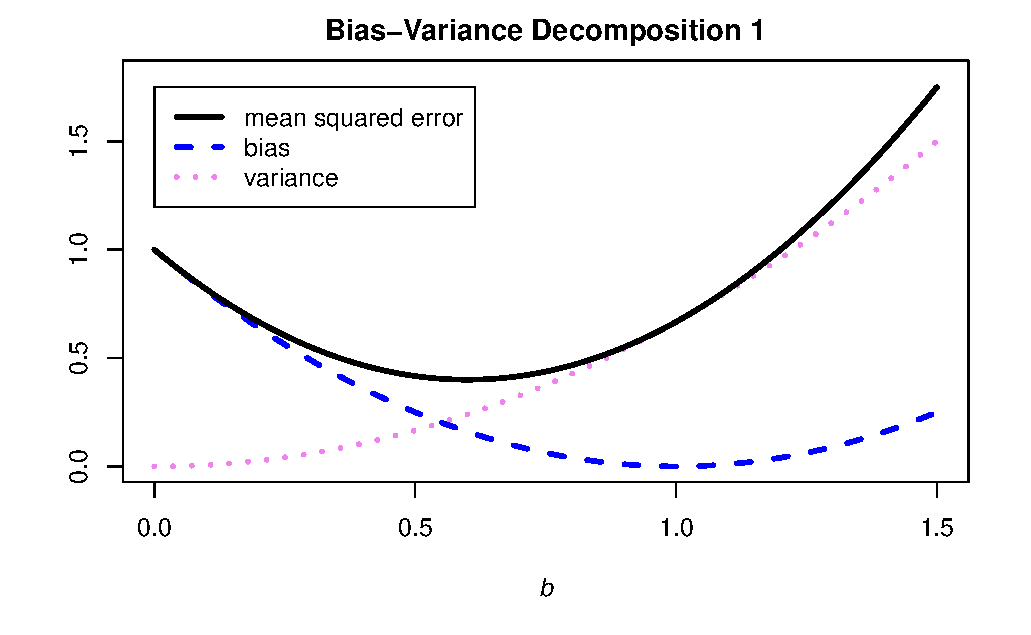
\includegraphics[scale=0.94]{bias-variance-decomposition-1.pdf}
    \caption{Plot of $b$ vs $\MSE(T_b, \sigma^2)$, $\Bias(T_b, \sigma^2)^2$, and $\Var T_b$ for $n=5$}
\end{figure}

\section{Density estimation}

\subsection{A point estimate}
Let $\cP$ be the set of all probability distributions that have smooth densities.
Since a smooth density characterizes a distribution uniquely (why?),
we can identify $\cP$ with the set of all smooth probability density functions on $\RR$:
\[
    \cP = \left\{f:\RR\to [0,\infty) :
    \text{$f$ is smooth and } \int_{-\infty}^\infty f(x)dx=1\right\}.
\]
Define a statistical functional $\theta$ on $\cP$ by rule
\[\theta(f)=f(0).\]

Let $X_1,\ldots,X_n\simiid f$ and let $h>0$. Then
\begin{align*}
    p_h &:= \Prob(|X_j|\leq h/2)\\ &= \int_{-h/2}^{h/2}f(x)\, dx\\
    &= \int_{-h/2}^{h/2} \left(f(0) + f'(0)x + \frac{f''(0)}2 x^2 + \frac{f'''(0)}6 h^3 + O(h^4)\right) dx\\
    &= f(0)h + \frac{f''(0)}{24}h^3 + O(h^5).
\end{align*}
    
Thus, for small $h$,
\[
    \EE \left[\frac{I(|X_j|\leq h/2)}h\right]\approx \theta(f).
\]
In particular, for small $h$,

This motivates considering
\[
    \hat\theta(X_1,\ldots,X_n) := \frac1{nh}\sum_{j=1}^nI(|X_j|\leq h/2)
\]
as an estimator of $\theta(f)$.
Then
\[
    \EE\theta(X_1,\ldots,X_n) = f(0) + \frac{f''(0)}{24}h^2 + O(h^3)
\]
and
\[
    \Bias(\hat\theta, \theta)^2 = \frac{f''(0)^2}{576}h^4 + O(h^6).
\]
As for the variance,
\begin{align*}
    \Var \hat\theta(X_1,\ldots,X_n) &= \frac1{n^2h^2}\sum_{j=1}^n \Var I(|X_j|\leq h/2)\\
    &= \frac1{n^2h^2}n p_h(1-p_h)\\
    &= \frac1{nh^2}\left(f(0)h - f(0)^2h^2 + \frac{f''(0)}{24}h^3 - \frac{f(0)f''(0)}{12}h^4 + \frac{f''(0)^2}{576}h^6\right)\\
    &= \frac1n\left(\frac{f(0)}h - f(0)^2 + \frac{f''(0)}{24}h - \frac{f(0)f''(0)}{12}h^2 + O(h^4)\right)
\end{align*}

\begin{figure}
    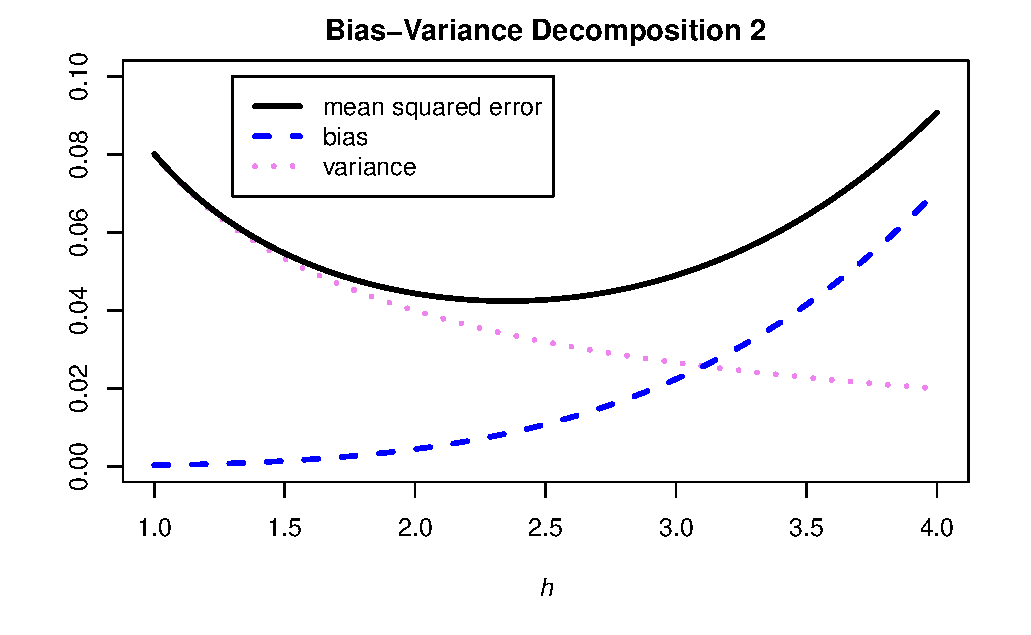
\includegraphics[scale=0.94]{bias-variance-decomposition-2.pdf}
    \caption{Plot of $b$ vs $\MSE(\hat\theta, \theta)$, $\Bias(\hat\theta, \theta)^2$, and $\Var \hat\theta$ for $n=5$}
\end{figure}


\subsection{The histogram estimator}

\section{The method of maximum likelihood}

$E[Y|X] = aX+b$

Suppose that 
\[
    Y = f(X)+\epsilon
\]
\end{document}